\section{Overall evaluation}
% Put games won/lost/tied as first/second player against other AIs here

The different optimisations described in the previous section were implemented in an incremental fashion (except for the asynchronous search, which wasn't applied to the agent with the artificial neural network). This gives us the following list of agents that we could test:
\begin{description}
	\item[Agent 1] Monte Carlo tree search
	\item[Agent 2] MCTS with early simulation termination
	\item[Agent 3] Agent 2 extended with reuse of the search tree
	\item[Agent 4] Agent 3 extended with the use of optimal moves
	\item[Agent 5] Agent 4 extended with asynchronous search
	\item[Agent 6] Agent 4 extended with ANN heuristic
\end{description}

To measure the difference in performance between the optimisations we made, we made the different agents compete with each other. All tested combinations of two different agents played 100 games of a given board size of 5x5 against each other. The player who starts first is alternated every game, to make it a fair comparison between the two agents.

\subsection{Agent 1 vs Agent 2}
First, the basic Monte Carlo tree search implementation competed with the optimisation that has early termination of simulation. 100 games were played on a board size of 5x5.

\begin{table}[!h]
	\centering
	\label{result:Ag1vsAg2}
	\begin{tabular}{c | c | c | c}
		& \multicolumn{3}{c}{\textbf{Winner}}        \\
		\textbf{Playing first} & Agent 1 & Tie & Agent 2 \\ \hline
		Agent 1 & 18 & 0 & 32 \\ \hline
		Agent 2 & 26 & 0 & 24
	\end{tabular}
	\caption{Agent 1 vs Agent 2}
\end{table}

\begin{figure}[!h]
	\centering
	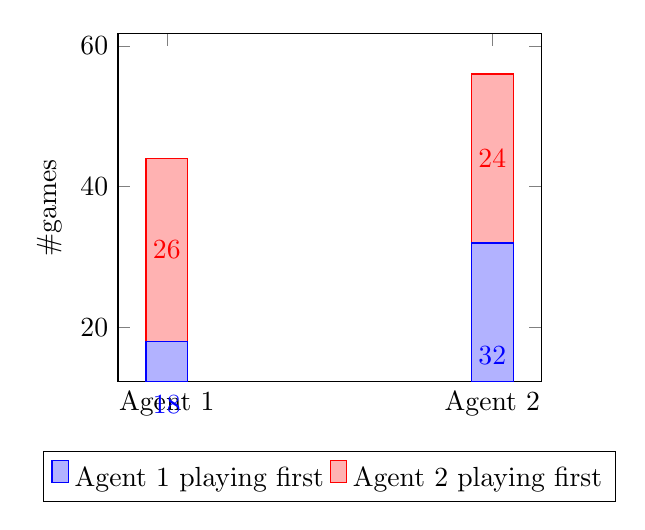
\begin{tikzpicture}
		\begin{axis}[
			ybar stacked,
			bar width=15pt,
			height=6cm,
			nodes near coords,
			enlargelimits=0.15,
			legend style={at={(0.5,-0.20)},
				anchor=north,legend columns=-1},
			ylabel={\#games},
			symbolic x coords={Agent 1, Agent 2},
			xtick=data,
			%x tick label style={rotate=45,anchor=east},
			]
			\addplot+[ybar] plot coordinates {(Agent 1, 18) (Agent 2, 32)};
			\addplot+[ybar] plot coordinates {(Agent 1, 26) (Agent 2, 24)};
			\legend{\strut Agent 1 playing first, \strut Agent 2 playing first}
		\end{axis}
	\end{tikzpicture}
	\caption{Agent 1 vs Agent 2: number of games won}
\end{figure}

\subsection{Agent 2 vs Agent 3}

\begin{table}[!h]
	\centering
	\label{result:Ag2vsAg3}
	\begin{tabular}{c | c | c | c}
		& \multicolumn{3}{c}{\textbf{Winner}}        \\
		\textbf{Playing first} & Agent 2 & Tie & Agent 3 \\ \hline
		Agent 2 & 25 & 0 & 25 \\ \hline
		Agent 3 & 22 & 0 & 28
	\end{tabular}
	\caption{Agent 2 vs Agent 3}
\end{table}

\begin{figure}[!h]
	\centering
	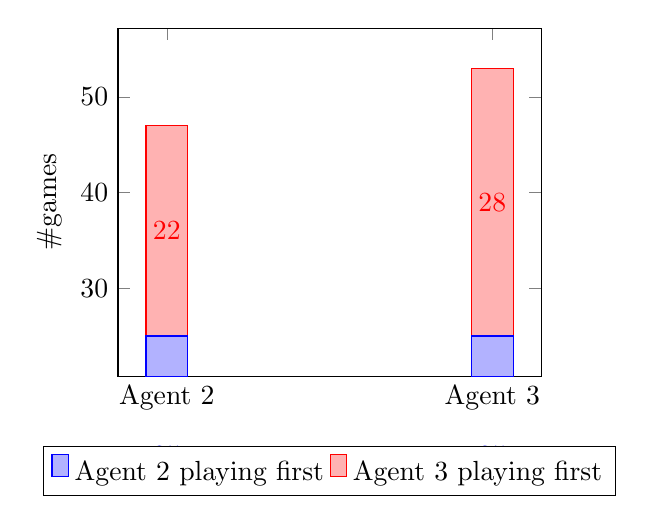
\begin{tikzpicture}
	\begin{axis}[
	ybar stacked,
	bar width=15pt,
	height=6cm,
	nodes near coords,
	enlargelimits=0.15,
	legend style={at={(0.5,-0.20)},
		anchor=north,legend columns=-1},
	ylabel={\#games},
	symbolic x coords={Agent 2, Agent 3},
	xtick=data,
	%x tick label style={rotate=45,anchor=east},
	]
	\addplot+[ybar] plot coordinates {(Agent 2, 25) (Agent 3, 25)};
	\addplot+[ybar] plot coordinates {(Agent 2, 22) (Agent 3, 28)};
	\legend{\strut Agent 2 playing first, \strut Agent 3 playing first}
	\end{axis}
	\end{tikzpicture}
	\caption{Agent 2 vs Agent 3: number of games won}
\end{figure}

\subsection{Agent 3 vs Agent 4}

\begin{table}[!h]
	\centering
	\label{result:Ag3vsAg4}
	\begin{tabular}{c | c | c | c}
		& \multicolumn{3}{c}{\textbf{Winner}}        \\
		\textbf{Playing first} & Agent 3 & Tie & Agent 4 \\ \hline
		Agent 3 & 0 & 0 & 50 \\ \hline
		Agent 4 & 50 & 0 & 0
	\end{tabular}
	\caption{Agent 3 vs Agent 4}
\end{table}

\begin{figure}[!h]
	\centering
	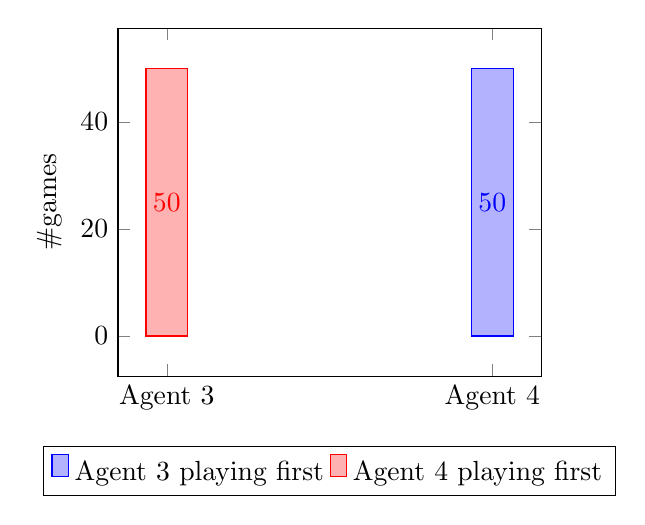
\begin{tikzpicture}
	\begin{axis}[
	ybar stacked,
	bar width=15pt,
	height=6cm,
	nodes near coords,
	enlargelimits=0.15,
	legend style={at={(0.5,-0.20)},
		anchor=north,legend columns=-1},
	ylabel={\#games},
	symbolic x coords={Agent 3, Agent 4},
	xtick=data,
	%x tick label style={rotate=45,anchor=east},
	]
	\addplot+[ybar] plot coordinates {(Agent 3, 0) (Agent 4, 50)};
	\addplot+[ybar] plot coordinates {(Agent 3, 50) (Agent 4, 0)};
	\legend{\strut Agent 3 playing first, \strut Agent 4 playing first}
	\end{axis}
	\end{tikzpicture}
	\caption{Agent 3 vs Agent 4: number of games won}
\end{figure}

\subsection{Agent 4 vs Agent 5}

\begin{table}[!h]
	\centering
	\label{result:Ag4vsAg5}
	\begin{tabular}{c | c | c | c}
		& \multicolumn{3}{c}{\textbf{Winner}}        \\
		\textbf{Playing first} & Agent 4 & Tie & Agent 5 \\ \hline
		Agent 4 & 30 & 0 & 20 \\ \hline
		Agent 5 & 25 & 0 & 25
	\end{tabular}
	\caption{Agent 4 vs Agent 5}
\end{table}

\begin{figure}[!h]
	\centering
	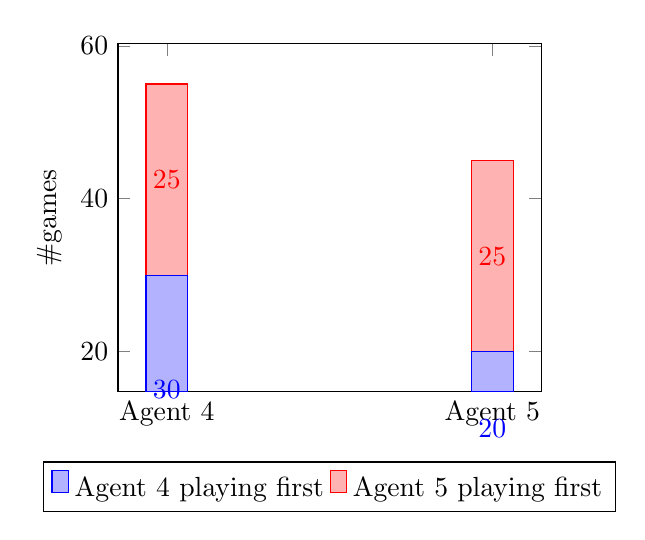
\begin{tikzpicture}
	\begin{axis}[
	ybar stacked,
	bar width=15pt,
	height=6cm,
	nodes near coords,
	enlargelimits=0.15,
	legend style={at={(0.5,-0.20)},
		anchor=north,legend columns=-1},
	ylabel={\#games},
	symbolic x coords={Agent 4, Agent 5},
	xtick=data,
	%x tick label style={rotate=45,anchor=east},
	]
	\addplot+[ybar] plot coordinates {(Agent 4, 30) (Agent 5, 20)};
	\addplot+[ybar] plot coordinates {(Agent 4, 25) (Agent 5, 25)};
	\legend{\strut Agent 4 playing first, \strut Agent 5 playing first}
	\end{axis}
	\end{tikzpicture}
	\caption{Agent 4 vs Agent 5: number of games won}
\end{figure}



\subsection{Agent 4 vs Agent 6}

\begin{table}[!h]
	\centering
	\label{result:Ag4vsAg6}
	\begin{tabular}{c | c | c | c}
		& \multicolumn{3}{c}{\textbf{Winner}}        \\
		\textbf{Playing first} & Agent 4 & Tie & Agent 6 \\ \hline
		Agent 4 & 25 & 0 & 25 \\ \hline
		Agent 6 & 25 & 0 & 25
	\end{tabular}
	\caption{Agent 4 vs Agent 6}
\end{table}

\begin{figure}[!h]
	\centering
	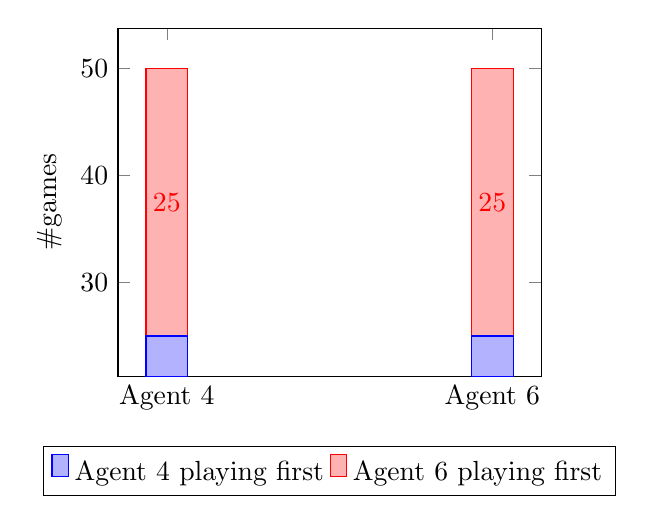
\begin{tikzpicture}
	\begin{axis}[
	ybar stacked,
	bar width=15pt,
	height=6cm,
	nodes near coords,
	enlargelimits=0.15,
	legend style={at={(0.5,-0.20)},
		anchor=north,legend columns=-1},
	ylabel={\#games},
	symbolic x coords={Agent 4, Agent 6},
	xtick=data,
	%x tick label style={rotate=45,anchor=east},
	]
	\addplot+[ybar] plot coordinates {(Agent 4, 25) (Agent 6, 25)};
	\addplot+[ybar] plot coordinates {(Agent 4, 25) (Agent 6, 25)};
	\legend{\strut Agent 4 playing first, \strut Agent 6 playing first}
	\end{axis}
	\end{tikzpicture}
	\caption{Agent 4 vs Agent 6: number of games won}
\end{figure}
